\documentclass[conference]{IEEEtran}
% QONTOS Research Paper Series — Shared LaTeX Preamble
% Use with: % QONTOS Research Paper Series — Shared LaTeX Preamble
% Use with: % QONTOS Research Paper Series — Shared LaTeX Preamble
% Use with: \input{qontos-preamble}

\usepackage{cite}
\usepackage{amsmath,amssymb,amsfonts}
\usepackage{graphicx}
\usepackage{textcomp}
\usepackage{xcolor}
\usepackage{hyperref}
\usepackage{booktabs}
\usepackage{multirow}
\usepackage{array}
\usepackage{tabularx}
\usepackage{float}
\usepackage{listings}
\usepackage{url}
\usepackage{enumitem}

% Listing style
\lstset{
  basicstyle=\ttfamily\footnotesize,
  breaklines=true,
  frame=single,
  backgroundcolor=\color{gray!10},
}

% Custom column type
\newcolumntype{L}[1]{>{\raggedright\arraybackslash}p{#1}}

% QONTOS colors
\definecolor{qontosnavy}{HTML}{0A1628}
\definecolor{qontosblue}{HTML}{1E88E5}
\definecolor{qontosteal}{HTML}{00BCD4}

% Hyperref setup
\hypersetup{
  colorlinks=true,
  linkcolor=qontosblue,
  citecolor=qontosblue,
  urlcolor=qontosteal,
}

% Author block
\newcommand{\qontosauthor}{%
\IEEEauthorblockN{QONTOS Research Wing}
\IEEEauthorblockA{
Zhyra Quantum Research Institute (ZQRI)\\
Advanced Quantum Systems Division\\
Abu Dhabi, UAE\\
\texttt{research@zhyra.xyz}}
}


\usepackage{cite}
\usepackage{amsmath,amssymb,amsfonts}
\usepackage{graphicx}
\usepackage{textcomp}
\usepackage{xcolor}
\usepackage{hyperref}
\usepackage{booktabs}
\usepackage{multirow}
\usepackage{array}
\usepackage{tabularx}
\usepackage{float}
\usepackage{listings}
\usepackage{url}
\usepackage{enumitem}

% Listing style
\lstset{
  basicstyle=\ttfamily\footnotesize,
  breaklines=true,
  frame=single,
  backgroundcolor=\color{gray!10},
}

% Custom column type
\newcolumntype{L}[1]{>{\raggedright\arraybackslash}p{#1}}

% QONTOS colors
\definecolor{qontosnavy}{HTML}{0A1628}
\definecolor{qontosblue}{HTML}{1E88E5}
\definecolor{qontosteal}{HTML}{00BCD4}

% Hyperref setup
\hypersetup{
  colorlinks=true,
  linkcolor=qontosblue,
  citecolor=qontosblue,
  urlcolor=qontosteal,
}

% Author block
\newcommand{\qontosauthor}{%
\IEEEauthorblockN{QONTOS Research Wing}
\IEEEauthorblockA{
Zhyra Quantum Research Institute (ZQRI)\\
Advanced Quantum Systems Division\\
Abu Dhabi, UAE\\
\texttt{research@zhyra.xyz}}
}


\usepackage{cite}
\usepackage{amsmath,amssymb,amsfonts}
\usepackage{graphicx}
\usepackage{textcomp}
\usepackage{xcolor}
\usepackage{hyperref}
\usepackage{booktabs}
\usepackage{multirow}
\usepackage{array}
\usepackage{tabularx}
\usepackage{float}
\usepackage{listings}
\usepackage{url}
\usepackage{enumitem}

% Listing style
\lstset{
  basicstyle=\ttfamily\footnotesize,
  breaklines=true,
  frame=single,
  backgroundcolor=\color{gray!10},
}

% Custom column type
\newcolumntype{L}[1]{>{\raggedright\arraybackslash}p{#1}}

% QONTOS colors
\definecolor{qontosnavy}{HTML}{0A1628}
\definecolor{qontosblue}{HTML}{1E88E5}
\definecolor{qontosteal}{HTML}{00BCD4}

% Hyperref setup
\hypersetup{
  colorlinks=true,
  linkcolor=qontosblue,
  citecolor=qontosblue,
  urlcolor=qontosteal,
}

% Author block
\newcommand{\qontosauthor}{%
\IEEEauthorblockN{QONTOS Research Wing}
\IEEEauthorblockA{
Zhyra Quantum Research Institute (ZQRI)\\
Advanced Quantum Systems Division\\
Abu Dhabi, UAE\\
\texttt{research@zhyra.xyz}}
}


\begin{document}

\title{Cryogenic Infrastructure Feasibility for Large-Scale Modular Quantum Systems}

\author{\qontosauthor}

\maketitle

\begin{abstract}
Cryogenic infrastructure is among the most consequential constraints on the path to million-qubit quantum computing. This paper reframes the cryogenic challenge as an infrastructure feasibility problem rather than a simple thermal-budget exercise. We present a scenario-banded analysis covering refrigeration plant architecture, wiring and control-electronics assumptions, maintenance and uptime modelling, failure-mode taxonomy, and facility-scale redundancy planning for modular superconducting quantum systems within the QONTOS programme. Our analysis draws on published specifications from commercial dilution-refrigerator platforms (Bluefors, Oxford Instruments Proteox) and the emerging literature on cryogenic CMOS control electronics. We identify the transition from single-refrigerator operation to facility-scale fleet management as the primary engineering cliff, and define validation gates that must be cleared before stretch-scenario claims can be promoted. All claims carry explicit status labels; no assumption is presented as demonstrated fact.

\textbf{Claim posture:} Infrastructure feasibility analysis. All projections carry scenario bands (Base / Aggressive / Stretch) and explicit claim labels.
\end{abstract}

\section{Introduction: Cryogenics as a First-Order System Constraint}

\subsection{Motivation and Scope}

The dominant narrative in quantum computing scaling focuses on qubit count, gate fidelity, and error-correction thresholds. In practice, the ability to cool, wire, control, and maintain modular quantum processors at millikelvin temperatures is equally decisive. A 100-module facility operating at 15~mK is not a scaled-up version of a single dilution refrigerator; it is an industrial cryogenic plant with its own failure modes, maintenance economics, and redundancy requirements.

This paper treats cryogenic infrastructure as a first-order feasibility question. We do not assume that cooling power alone determines viability. Instead, we model the full thermal stack---from qubit-chip dissipation through wiring heat loads, control-electronics staging, refrigerator architecture, and facility-level fleet management---and identify the conditions under which each scenario band remains physically and operationally credible.

\textbf{[Claim: CRYO-01 $|$ Demonstrated]} Dilution refrigerators routinely achieve base temperatures below 10~mK with cooling powers of 10--25~$\mu$W at 20~mK in single-unit laboratory configurations~\cite{Krinner2019}.

\textbf{[Claim: CRYO-02 $|$ Engineering extrapolation]} Scaling to multi-refrigerator facilities of 10--100 units introduces qualitatively new constraints in maintenance scheduling, redundancy, and thermal-load management that have no direct laboratory precedent.

\subsection{Claim Status Summary}

\begin{table}[H]
\centering
\caption{Claim status summary for cryogenic infrastructure.}
\label{tab:claim-summary}
\footnotesize
\begin{tabularx}{\columnwidth}{lL{3.0cm}L{2.5cm}}
\toprule
\textbf{ID} & \textbf{Statement} & \textbf{Status} \\
\midrule
CRYO-01 & Single-unit DR cooling at 15~mK sufficient for current modules & Demonstrated \\
CRYO-02 & Multi-unit facility introduces new engineering constraints & Eng.\ extrapolation \\
CRYO-03 & 25~mW per module at MXC achievable & Aggressive target \\
CRYO-04 & 100-module facility with 95\% uptime feasible & Stretch---unvalidated \\
CRYO-05 & Cryo-CMOS reduces wiring 5--10$\times$ & Research projection \\
CRYO-06 & Photonic interconnects reduce inter-module thermal load $>$90\% vs coaxial & Arch.-dependent projection \\
\bottomrule
\end{tabularx}
\end{table}

\subsection{Wiring and Control-Electronics Assumptions}

The thermal feasibility of any modular quantum architecture is dominated not by qubit dissipation but by the wiring and control infrastructure required to operate qubits. This subsection makes those assumptions explicit.

\textbf{Control-line taxonomy per module (stretch scenario, 1,000-qubit module):}

\begin{table}[H]
\centering
\caption{Control-line heat load per module at MXC stage.}
\label{tab:control-lines}
\footnotesize
\begin{tabularx}{\columnwidth}{L{1.8cm}rrrL{1.8cm}}
\toprule
\textbf{Line type} & \textbf{Count} & \textbf{Heat/line} & \textbf{Total} & \textbf{Source} \\
\midrule
Coax RF drive & 200 & 50~$\mu$W & 10.0~mW & \cite{Krinner2019} \\
Coax RF readout & 100 & 50~$\mu$W & 5.0~mW & \cite{Krinner2019} \\
DC bias (filtered) & 200 & 1~$\mu$W & 0.2~mW & \cite{Reilly2015} \\
Flux-tuning & 100 & 10~$\mu$W & 1.0~mW & \cite{Krinner2019} \\
HEMT amp.\ (4~K) & 10 & -- & see 4~K & \cite{Hornibrook2015} \\
Optical fibres & 20 & 0.5~$\mu$W & 0.01~mW & Arch.\ projection \\
\midrule
\textbf{Total at MXC} & & & \textbf{$\sim$16.2~mW} & \\
\bottomrule
\end{tabularx}
\end{table}

\textbf{[Claim: CRYO-07 $|$ Engineering estimate]} The wiring heat-load budget above assumes conventional coaxial attenuation schemes. Cryogenic CMOS multiplexing~\cite{Bardin2019, Pauka2021} could reduce the coaxial line count by 5--10$\times$, bringing the MXC load below 5~mW per module. This reduction is not assumed in the base or aggressive scenarios.

\textbf{Attenuation and filtering strategy:} Each RF line requires 60~dB of total attenuation distributed across temperature stages to suppress room-temperature Johnson noise. A standard staging distributes attenuators at 50~K (20~dB), 4~K (20~dB), and MXC (20~dB), with the heat dissipated at each stage proportional to the attenuation ratio and the input power. The MXC-stage attenuation dominates the thermal budget because cooling power at 15~mK is five to six orders of magnitude more expensive per watt than at 4~K~\cite{Krinner2019}.

\textbf{Electronics staging assumptions:}

\begin{table}[H]
\centering
\caption{Electronics staging across temperature stages.}
\label{tab:electronics-staging}
\footnotesize
\begin{tabularx}{\columnwidth}{L{1.3cm}rL{2.5cm}r}
\toprule
\textbf{Stage} & \textbf{Temp.} & \textbf{Components} & \textbf{Heat budget} \\
\midrule
Room temp. & 300~K & AWGs, digitisers, classical compute & Unlimited (HVAC) \\
50~K & 50~K & First-stage atten., thermal anchoring & 10--40~W \\
4~K & 4~K & HEMT amps, cryo-CMOS (future) & 1--2~W/module \\
Still & 800~mK & Secondary filtering, thermal intercepts & 100--500~mW \\
MXC & 15~mK & QPU, final atten., JPA & 10--25~mW/module \\
\bottomrule
\end{tabularx}
\end{table}

The 4~K stage is the critical bottleneck for future cryo-CMOS integration. Bardin et al.~\cite{Bardin2019} demonstrated a 28~nm bulk-CMOS controller dissipating approximately 2~mW per qubit at 3~K. Pauka et al.~\cite{Pauka2021} demonstrated a cryo-CMOS chip generating control signals for multiple qubits at power levels compatible with the 4~K stage of a commercial DR. Van~Dijk et al.~\cite{VanDijk2019} provide a comprehensive review of the electronic interface requirements for quantum processors and identify the 4~K power budget as the binding constraint for integrated control.

\section{Refrigeration Plant Architecture and Facility Model}

\begin{figure}[t]
\centering
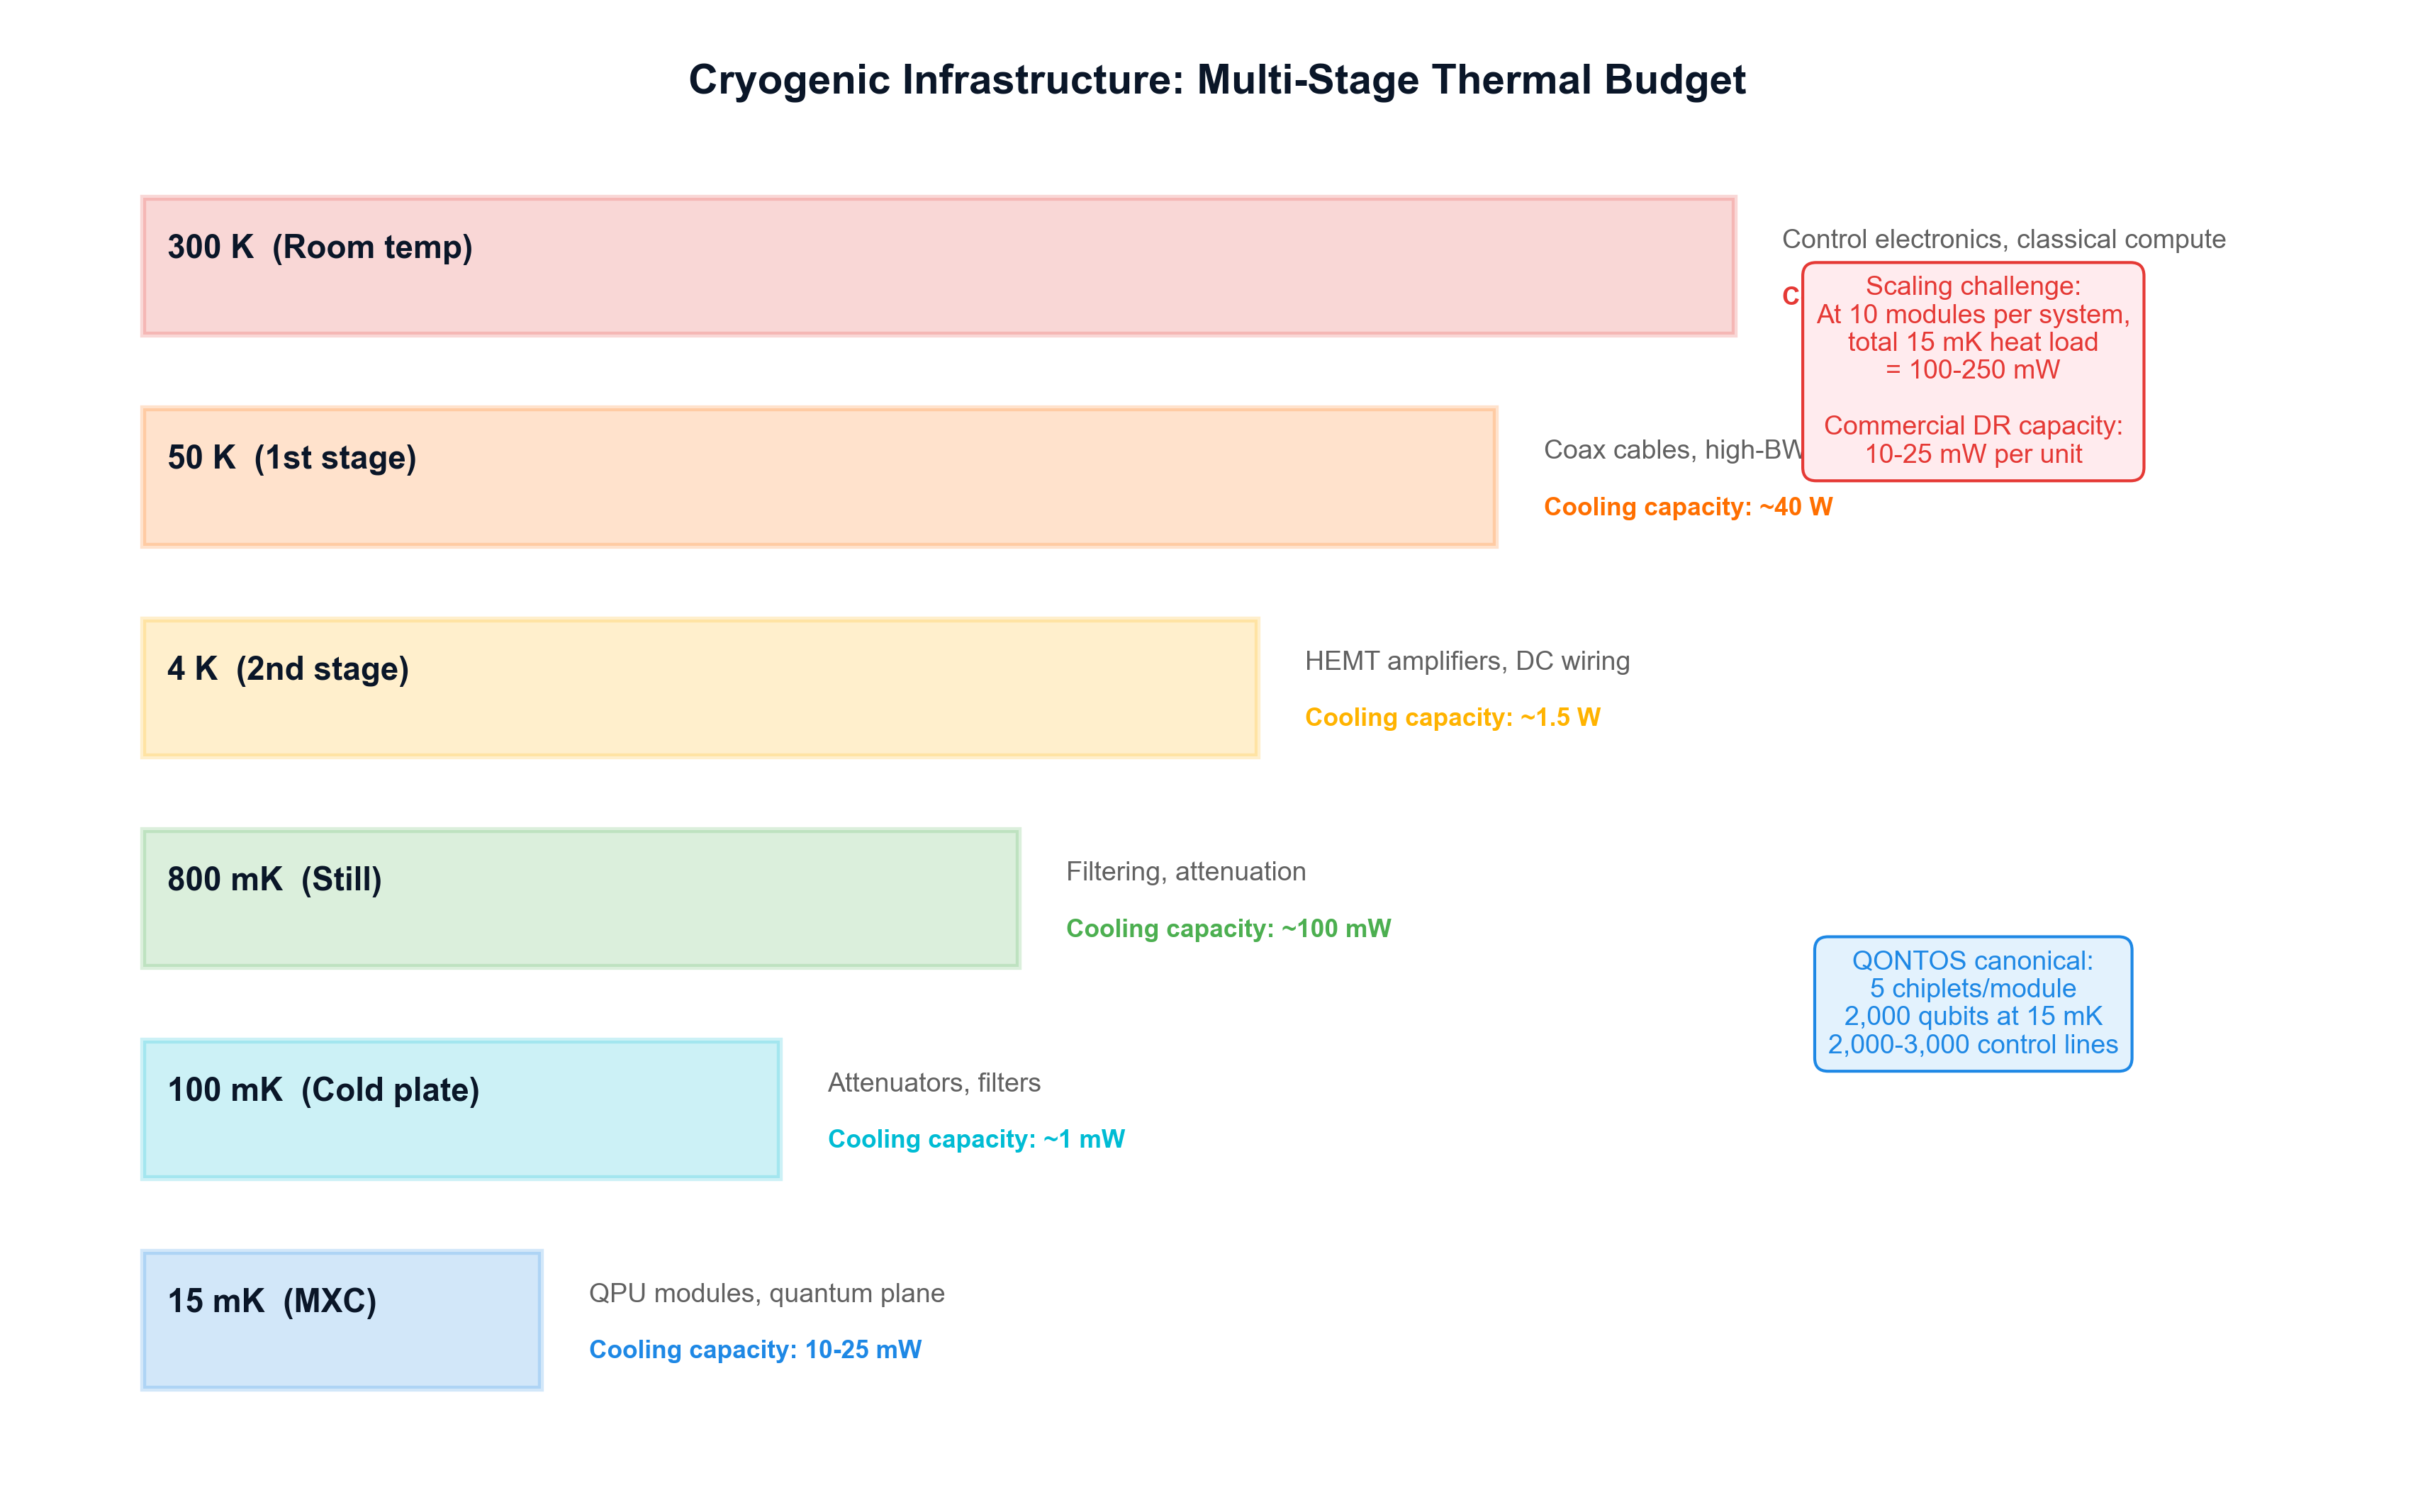
\includegraphics[width=\columnwidth]{../../figures/07_cryogenic.png}
\caption{Cryogenic thermal budget overview for the QONTOS modular architecture.}
\label{fig:cryogenic}
\end{figure}

The cryogenic infrastructure supports both the superconducting processor modules and their photonic interconnect interfaces. The hybrid superconducting-photonic architecture imposes thermal requirements at multiple stages: the superconducting qubits operate at millikelvin temperatures while the photonic transduction and interconnect components introduce their own thermal loads at intermediate stages.

\subsection{Refrigeration Plant Architecture}

\textbf{Single-unit baseline (Base scenario):} Commercial dilution refrigerators from Bluefors (LD and XLD series) and Oxford Instruments (Proteox) provide the baseline capability. Published specifications indicate:

\begin{itemize}
\item Bluefors XLD series: base temperature $<$~8~mK, cooling power $>$~20~$\mu$W at 20~mK, sample space diameter up to 400~mm, pre-cool time approximately 24--36 hours~\cite{Bluefors}.
\item Oxford Instruments Proteox: base temperature $<$~5~mK, modular insert architecture allowing sample exchange without full warm-up, cooling power approximately 15~$\mu$W at 20~mK~\cite{OxfordProteox}.
\end{itemize}

\textbf{[Claim: CRYO-08 $|$ Demonstrated]} Both platforms have been deployed in multi-qubit experiments worldwide and represent the current engineering baseline for superconducting quantum computing.

\textbf{Multi-unit facility architecture (Aggressive and Stretch scenarios):}

\begin{table}[H]
\centering
\caption{Multi-unit facility parameters by scenario.}
\label{tab:facility-params}
\footnotesize
\begin{tabularx}{\columnwidth}{L{2.5cm}rrr}
\toprule
\textbf{Parameter} & \textbf{Base (10)} & \textbf{Aggr.\ (50)} & \textbf{Stretch (100)} \\
\midrule
Refrigerator units & 10 & 50 + 5 spare & 100 + 10 spare \\
Cooling/mod.\ at MXC & 10~mW & 20~mW & 25~mW \\
Total MXC capacity & 100~mW & 1,000~mW & 2,500~mW \\
Facility elec.\ power & 150--300~kW & 500--750~kW & 1.0--1.5~MW \\
He-3 inventory & 10--30~L & 50--150~L & 100--300~L \\
Floor area (cryo hall) & 200~m$^2$ & 800~m$^2$ & 1,500--2,000~m$^2$ \\
Cooling-water req. & 50~kW & 250~kW & 500~kW \\
\bottomrule
\end{tabularx}
\end{table}

\textbf{[Claim: CRYO-09 $|$ Aggressive planning target]} A 50-unit facility is within the envelope of industrial cryogenic installations (e.g.\ large-scale MRI or particle-physics facilities) but has never been built for quantum computing. The primary unknowns are vibration isolation at density, helium-3 supply-chain risk, and coordinated maintenance scheduling.

\textbf{[Claim: CRYO-10 $|$ Stretch assumption---unvalidated]} A 100-unit facility with 25~mW per module at MXC requires cooling-power specifications approximately 25\% beyond the published performance of current commercial platforms. This gap may be closed by next-generation DR designs, but no public datasheet currently validates 25~mW at 15~mK.

\textbf{Helium-3 supply-chain considerations:} Each dilution refrigerator requires 1--3 litres of helium-3 in its mixture. At current market prices (approximately USD~2,000--3,000 per litre) and constrained global supply (primarily from tritium decay in nuclear facilities), a 100-unit facility represents a helium-3 inventory valued at USD~200k--900k with non-trivial procurement lead times. This is a logistical constraint, not a feasibility barrier, but it must be planned.

\subsection{Maintenance and Uptime Model}

\textbf{Maintenance taxonomy:}

\begin{table}[H]
\centering
\caption{Maintenance event taxonomy for dilution refrigerators.}
\label{tab:maintenance}
\footnotesize
\begin{tabularx}{\columnwidth}{L{1.8cm}rL{1.5cm}L{1.8cm}}
\toprule
\textbf{Event type} & \textbf{Duration} & \textbf{Frequency} & \textbf{Impact} \\
\midrule
Routine sensor cal. & 2--4~h & Monthly & No warm-up \\
Insert exchange & 4--8~h & As needed & Partial warm-up to 4~K \\
Full thermal cycle & 48--72~h & 1--2/year & Unit offline 3+ days \\
Compressor maint. & 4--8~h & Annual & Unit offline \\
Leak repair & 24--120~h & $<$0.1/unit-yr & Extended downtime \\
Pulse-tube replace. & 8--24~h & Every 3--5~yr & Unit offline (plannable) \\
\bottomrule
\end{tabularx}
\end{table}

\textbf{Uptime model by scenario:}

\begin{table}[H]
\centering
\caption{Uptime model by scenario band.}
\label{tab:uptime}
\footnotesize
\begin{tabularx}{\columnwidth}{L{1.3cm}L{1.2cm}L{1.2cm}rrr}
\toprule
\textbf{Scen.} & \textbf{Planned DT} & \textbf{Unplanned DT} & \textbf{Gross} & \textbf{W/ redund.} & \textbf{Net} \\
\midrule
Base & 15~d & 10~d & 90.4\% & N/A & $\sim$90\% \\
Aggr. & 10~d & 7~d & 95.3\% & 10\% spare & $\sim$93\% \\
Stretch & 7~d & 5~d & 96.7\% & 10\%+swap & $\sim$95\% \\
\bottomrule
\end{tabularx}
\end{table}

\textbf{[Claim: CRYO-11 $|$ Aggressive planning target]} Achieving 93\% net effective uptime across a 50-unit fleet requires a maintenance-scheduling system that staggers thermal cycles, maintains a 10\% spare fleet, and completes unplanned repairs within a mean time to repair (MTTR) of 72~hours.

\textbf{[Claim: CRYO-12 $|$ Stretch assumption---unvalidated]} 95\% net effective uptime across 100 units assumes hot-swappable module inserts, a dedicated cryogenic-engineering team of 10--15 FTEs, and predictive-maintenance instrumentation on every unit. No quantum-computing facility has demonstrated this operational model.

\textbf{Staffing model:}

\begin{table}[H]
\centering
\caption{Cryogenic operations staffing model.}
\label{tab:staffing}
\footnotesize
\begin{tabularx}{\columnwidth}{lrrr}
\toprule
\textbf{Scenario} & \textbf{Cryo engineers} & \textbf{Technicians} & \textbf{Total FTEs} \\
\midrule
Base (10 units) & 2 & 3 & 5 \\
Aggressive (50 units) & 4 & 8 & 12 \\
Stretch (100 units) & 6 & 12 & 18 \\
\bottomrule
\end{tabularx}
\end{table}

\subsection{Failure Modes}

A rigorous feasibility analysis requires explicit enumeration of failure modes that could invalidate scenario assumptions. We organize these by severity and probability.

\textbf{Category A---High severity, moderate probability (facility-level risk):}

\begin{table}[H]
\centering
\caption{Category~A failure modes: facility-level risk.}
\label{tab:fm-a}
\footnotesize
\begin{tabularx}{\columnwidth}{cL{2.0cm}L{1.8cm}L{2.0cm}}
\toprule
\textbf{ID} & \textbf{Mechanism} & \textbf{Consequence} & \textbf{Mitigation} \\
\midrule
FM-A1 & Wiring density exceeds thermal margin & Module thermally infeasible & Cryo-CMOS mux; photonic readout \\
FM-A2 & Correlated fleet failures & Uptime collapses & Spare fleet; staggered procurement \\
FM-A3 & He-3 supply disruption & Cannot charge/repair units & Strategic reserve; closed-loop recovery \\
\bottomrule
\end{tabularx}
\end{table}

\textbf{Category B---High severity, low probability (design-level risk):}

\begin{table}[H]
\centering
\caption{Category~B failure modes: design-level risk.}
\label{tab:fm-b}
\footnotesize
\begin{tabularx}{\columnwidth}{cL{2.0cm}L{1.8cm}L{2.0cm}}
\toprule
\textbf{ID} & \textbf{Mechanism} & \textbf{Consequence} & \textbf{Mitigation} \\
\midrule
FM-B1 & Vibration coupling at scale & Correlated decoherence & Isolated foundations; active damping \\
FM-B2 & EMI at density & Gate-error floors rise & Shielded cabling; Faraday enclosures \\
FM-B3 & Cryo-CMOS reliability at scale & Increased downtime & Accelerated life testing; dual-path arch. \\
\bottomrule
\end{tabularx}
\end{table}

\textbf{Category C---Moderate severity, high probability (operational risk):}

\begin{table}[H]
\centering
\caption{Category~C failure modes: operational risk.}
\label{tab:fm-c}
\footnotesize
\begin{tabularx}{\columnwidth}{cL{2.0cm}L{1.8cm}L{2.0cm}}
\toprule
\textbf{ID} & \textbf{Mechanism} & \textbf{Consequence} & \textbf{Mitigation} \\
\midrule
FM-C1 & Calibration drift post-thermal-cycle & Hours--days recalibration & Automated recal.\ protocols \\
FM-C2 & Operator error in fleet mgmt. & Temporary capacity loss & SW-managed orchestration; interlocks \\
FM-C3 & Cooling-water/power interruption & All units begin warming & UPS; thermal-inertia design \\
\bottomrule
\end{tabularx}
\end{table}

\subsection{Validation Gates}

The cryogenic infrastructure thesis must clear specific validation gates before scenario claims can be promoted. These gates are ordered by dependency; each must be satisfied before subsequent gates become meaningful.

\textbf{Gate V1---Wiring and Thermal Budget Closure (required for Base promotion):}
\begin{itemize}
\item Complete wiring manifest for a single module (all line types, attenuator placements, thermal anchoring)
\item Measured heat load at each temperature stage consistent with planned DR capacity
\item Demonstrated base temperature $<$~15~mK with full wiring installed
\item Status: Partially demonstrated in laboratory settings~\cite{Krinner2019, Hornibrook2015}
\end{itemize}

\textbf{Gate V2---Control-Electronics Architecture (required for Aggressive promotion):}
\begin{itemize}
\item Defined electronics staging plan (room temperature vs.\ 4~K vs.\ MXC)
\item If cryo-CMOS is assumed: demonstrated controller at 4~K with power dissipation within 4~K stage budget
\item Measured qubit performance ($T_1$, $T_2$, gate fidelity) with chosen electronics architecture
\item Status: Early demonstrations exist~\cite{Bardin2019, Pauka2021}; integration with full module not yet published
\end{itemize}

\textbf{Gate V3---Multi-Unit Fleet Operations (required for Aggressive promotion):}
\begin{itemize}
\item Demonstrated simultaneous operation of $\geq$~5 dilution refrigerators with coordinated maintenance scheduling
\item Measured vibration and EMI cross-coupling between adjacent units
\item Validated spare-unit failover procedure (module transfer to spare DR within 48~hours)
\item Status: No public demonstration in quantum-computing context
\end{itemize}

\textbf{Gate V4---Facility-Scale Uptime (required for Stretch promotion):}
\begin{itemize}
\item 12-month operational record of $\geq$~20 units with measured uptime $\geq$~90\%
\item Demonstrated predictive-maintenance system reducing unplanned downtime by $\geq$~30\%
\item Validated He-3 recovery and recycling system with $<$~5\% annual loss rate
\item Status: Not yet attempted
\end{itemize}

\textbf{Gate V5---Economic Viability (required for Stretch promotion):}
\begin{itemize}
\item Total cost of ownership (TCO) model for 100-unit facility over 10-year horizon
\item TCO per logical-qubit-hour competitive with alternative architectures (ion trap, photonic, neutral atom)
\item Status: No public TCO model exists for this scale
\end{itemize}

\section{Scenario-Based Thermal Envelope}

\subsection{Module-Level Thermal Budget}

The thermal budget at each cryogenic stage determines whether a given module design is physically operable. We present the stretch-scenario budget as the most constraining case.

\textbf{Stretch scenario---per-module thermal budget at MXC (15~mK):}

\begin{table}[H]
\centering
\caption{Per-module thermal budget at MXC (stretch scenario).}
\label{tab:thermal-budget}
\footnotesize
\begin{tabularx}{\columnwidth}{L{3.0cm}rL{2.5cm}}
\toprule
\textbf{Component} & \textbf{Heat load} & \textbf{Notes} \\
\midrule
Coaxial RF lines (300) & 15.0~mW & 50~$\mu$W/line~\cite{Krinner2019} \\
DC bias \& flux lines (300) & 1.2~mW & 1--10~$\mu$W/line~\cite{Reilly2015} \\
Optical fibres (20) & 0.01~mW & Negligible conductivity \\
On-chip dissipation (QPU) & 0.5~mW & Duty-cycle dependent \\
Josephson param.\ amps & 0.2~mW & Pump-tone leakage \\
Structural conduction & 1.0~mW & Mechanical design dependent \\
\midrule
\textbf{Total planned load} & \textbf{$\sim$17.9~mW} & \\
\textbf{Available cooling} & \textbf{25~mW} & CRYO-03: aggressive target \\
\textbf{Thermal margin} & \textbf{$\sim$7.1~mW (28\%)} & Min.\ recommended: 20\% \\
\bottomrule
\end{tabularx}
\end{table}

\textbf{[Claim: CRYO-13 $|$ Aggressive planning target]} The 28\% thermal margin is adequate for the stretch scenario only if wiring counts do not grow beyond the values assumed above. Every additional 100 coaxial lines adds approximately 5~mW to the MXC load, consuming the margin entirely.

\textbf{With cryo-CMOS multiplexing (projected):}

\begin{table}[H]
\centering
\caption{Per-module thermal budget with cryo-CMOS multiplexing.}
\label{tab:thermal-cryocmos}
\footnotesize
\begin{tabularx}{\columnwidth}{L{3.2cm}rL{2.5cm}}
\toprule
\textbf{Component} & \textbf{Heat load} & \textbf{Notes} \\
\midrule
Coaxial RF (reduced to 60) & 3.0~mW & 5$\times$ reduction~\cite{Bardin2019, VanDijk2019} \\
DC/flux lines (reduced to 60) & 0.24~mW & Multiplexed at 4~K \\
Cryo-CMOS at 4~K & -- & 0.5--2.0~W at 4~K (not MXC) \\
Other loads & 1.71~mW & Unchanged \\
\midrule
\textbf{Total planned load} & \textbf{$\sim$4.95~mW} & \\
\textbf{Available cooling} & \textbf{25~mW} & \\
\textbf{Thermal margin} & \textbf{$\sim$20~mW (80\%)} & \\
\bottomrule
\end{tabularx}
\end{table}

\textbf{[Claim: CRYO-05 $|$ Research projection]} Cryo-CMOS multiplexing transforms the MXC thermal budget from tight to comfortable, but shifts the bottleneck to the 4~K stage, which must absorb 0.5--2.0~W of additional dissipation per module. This is within pulse-tube capacity for current DR platforms but has not been demonstrated at module scale.

\subsection{Facility-Level Thermal Envelope}

\begin{table}[H]
\centering
\caption{Facility-level thermal envelope by scenario.}
\label{tab:facility-thermal}
\footnotesize
\begin{tabularx}{\columnwidth}{L{2.8cm}rrr}
\toprule
\textbf{Parameter} & \textbf{Base} & \textbf{Aggr.} & \textbf{Stretch} \\
\midrule
Modules & 10 & 50 & 100 \\
MXC cooling/module & 10~mW & 20~mW & 25~mW \\
Total MXC capacity & 100~mW & 1,000~mW & 2,500~mW \\
4~K load/module & 0.5~W & 1.0~W & 1.5~W \\
Total 4~K capacity & 5~W & 50~W & 150~W \\
50~K load/module & 5~W & 10~W & 15~W \\
Total 50~K capacity & 50~W & 500~W & 1,500~W \\
Facility elec.\ power & 150~kW & 600~kW & 1.2~MW \\
Facility cooling-water & 50~kW & 200~kW & 400~kW \\
\bottomrule
\end{tabularx}
\end{table}

\section{Photonic Interconnects and Thermal Impact}

Photonic interconnects between modules are analysed in detail in the companion paper (QONTOS Paper~04). Their relevance to cryogenic infrastructure is specifically thermal: optical fibres carry negligible heat compared with coaxial cables, and photonic transduction may eliminate entire categories of inter-module RF wiring.

\textbf{Thermal comparison---inter-module link:}

\begin{table}[H]
\centering
\caption{Thermal load comparison for inter-module link types.}
\label{tab:link-thermal}
\footnotesize
\begin{tabularx}{\columnwidth}{L{2.5cm}rrr}
\toprule
\textbf{Link type} & \textbf{Heat/link at MXC} & \textbf{Links/pair} & \textbf{Total/pair} \\
\midrule
Coaxial (semi-rigid) & 50--100~$\mu$W & 10--50 & 0.5--5.0~mW \\
Optical fibre (SM) & 0.1--1.0~$\mu$W & 10--50 & 0.001--0.05~mW \\
\textbf{Reduction factor} & & & \textbf{100--1,000$\times$} \\
\bottomrule
\end{tabularx}
\end{table}

\textbf{[Claim: CRYO-06 $|$ Architecture-dependent projection]} If photonic interconnects replace coaxial inter-module links, the inter-module thermal contribution at MXC drops from a significant fraction of the budget to negligible. This is a strong motivation for the photonic-interconnect programme, but the transduction hardware (microwave-to-optical conversion) introduces its own heat load at the 4~K or still stage, which is not yet fully characterised.

\section{Redundancy and Facility Operations Model}

\subsection{Redundancy Architecture}

The stretch scenario assumes that not all 100 refrigerators need to be simultaneously operational. A redundancy model with N+M architecture (N active, M spare) allows maintenance without reducing computational capacity below the threshold required for error-corrected operation.

\begin{table}[H]
\centering
\caption{Redundancy architecture by scenario.}
\label{tab:redundancy}
\footnotesize
\begin{tabularx}{\columnwidth}{lrrrr}
\toprule
\textbf{Scenario} & \textbf{Active (N)} & \textbf{Spare (M)} & \textbf{Ratio} & \textbf{Min.\ for full op.} \\
\midrule
Base & 10 & 0 & 0\% & 10 (no redundancy) \\
Aggressive & 50 & 5 & 10\% & 45 (graceful degrad.) \\
Stretch & 100 & 10 & 10\% & 90 (graceful degrad.) \\
\bottomrule
\end{tabularx}
\end{table}

\textbf{[Claim: CRYO-14 $|$ Aggressive planning target]} The 10\% spare ratio is borrowed from data-centre practices for critical infrastructure. Whether quantum error correction can tolerate the loss of 10\% of physical modules depends on the logical-qubit encoding and the inter-module connectivity graph, which is analysed in the companion error-correction paper (QONTOS Paper~03).

\subsection{Fleet Orchestration}

Managing 100+ dilution refrigerators requires software-managed fleet orchestration analogous to data-centre management platforms. Key requirements include:

\begin{itemize}
\item \textbf{Staggered thermal cycling:} No more than 5\% of units undergoing simultaneous warm-up to maintain facility cooling-water and power headroom.
\item \textbf{Predictive diagnostics:} Continuous monitoring of mixture pressure, pulse-tube vibration spectrum, and temperature stability to predict failures 48--72~hours in advance.
\item \textbf{Automated failover:} When a unit enters unplanned downtime, the orchestration system reassigns its computational workload to spare units and initiates module transfer if the architecture supports hot-swap.
\item \textbf{He-3 inventory tracking:} Real-time accounting of helium-3 across all units, recovery systems, and strategic reserve.
\end{itemize}

\subsection{Facility Layout Considerations}

A 100-unit cryogenic facility requires careful physical planning:

\begin{itemize}
\item \textbf{Vibration isolation:} Each DR requires its own vibration-isolated foundation. Minimum centre-to-centre spacing of 2.5--3.0~m is recommended based on acoustic coupling measurements in multi-DR laboratories.
\item \textbf{Utilities distribution:} Cooling water, compressed helium, electrical power, and signal cabling must be routed to each unit with sufficient redundancy and isolation to prevent single-point failures.
\item \textbf{Access for maintenance:} Each unit must be accessible from at least three sides for cryogenic maintenance. This sets a minimum aisle width of 1.5~m.
\item \textbf{RF shielding:} The facility requires either per-unit Faraday cages or a facility-wide shielded room to prevent electromagnetic interference between units and from external sources.
\end{itemize}

\section{Economic Framing}

While a full cost model is beyond the scope of this paper, we provide order-of-magnitude framing to contextualise feasibility.

\begin{table}[H]
\centering
\caption{Order-of-magnitude cost framing for a 100-unit facility.}
\label{tab:cost}
\footnotesize
\begin{tabularx}{\columnwidth}{L{3.0cm}rr}
\toprule
\textbf{Cost element} & \textbf{Per unit} & \textbf{100-unit facility} \\
\midrule
Dilution refrigerator & USD~500k--1M & USD~50--100M \\
Wiring \& MW components & USD~100--200k & USD~10--20M \\
Room-temp.\ electronics & USD~200--500k & USD~20--50M \\
Facility construction & -- & USD~20--40M \\
He-3 inventory & USD~3--9k & USD~300--900k \\
Annual ops (staff, util., maint.) & USD~50--100k & USD~5--10M/yr \\
\midrule
\textbf{10-year TCO (OoM)} & & \textbf{USD~150--300M} \\
\bottomrule
\end{tabularx}
\end{table}

\textbf{[Claim: CRYO-15 $|$ Order-of-magnitude estimate]} These figures are based on publicly available pricing for commercial DR platforms and standard industrial facility costs. They do not include QPU fabrication, classical computing infrastructure, or software development. The per-logical-qubit-hour cost depends critically on qubit count per module, error-correction overhead, and utilisation rate---all of which are analysed in companion papers.

\section{Synthesis and Risk Assessment}

\subsection{Scenario Viability Summary}

\begin{table}[H]
\centering
\caption{Scenario viability summary across key dimensions.}
\label{tab:viability}
\footnotesize
\begin{tabularx}{\columnwidth}{L{1.5cm}L{1.8cm}L{1.8cm}L{1.8cm}}
\toprule
\textbf{Dimension} & \textbf{Base (10)} & \textbf{Aggr.\ (50)} & \textbf{Stretch (100)} \\
\midrule
Thermal budget & Demonstrated & Feasible w/ margin & Requires next-gen DR or cryo-CMOS \\
Wiring & Standard practice & Dense but manageable & Cryo-CMOS likely required \\
Maint./uptime & Lab-scale ops & Fleet mgmt.\ needed & Industrial-scale ops \\
Redundancy & None required & 10\% spare fleet & 10\% spare + hot-swap \\
Facility infra. & Standard lab & Dedicated cryo hall & Purpose-built facility \\
Economic & Lab budgets & Major capital prog. & USD~150--300M TCO \\
Validation & Partially demo. & Gates V1--V2 & Gates V1--V5 all req. \\
\bottomrule
\end{tabularx}
\end{table}

\subsection{Critical Path Items}

\begin{enumerate}
\item \textbf{Wiring budget closure (Gate V1):} The single most important near-term activity. Without a validated wiring manifest, all thermal projections are provisional.
\item \textbf{Cryo-CMOS integration (Gate V2):} Determines whether the stretch scenario is thermally feasible without next-generation DR hardware.
\item \textbf{Multi-unit operations demonstration (Gate V3):} The transition from single-unit lab operation to fleet management is the least characterised engineering risk.
\item \textbf{He-3 supply strategy:} Not technically difficult but requires early procurement planning given 12--18 month lead times.
\end{enumerate}

\subsection{What Would Change Our Assessment}

\begin{itemize}
\item \textbf{Upward revision:} A demonstrated cryo-CMOS controller operating reliably at 4~K with $<$~1~W per 1,000 qubits would make the stretch scenario thermally comfortable and shift the primary constraint to facility operations.
\item \textbf{Upward revision:} A DR platform with validated $>$~30~mW cooling power at 15~mK would provide sufficient margin for the stretch scenario even without cryo-CMOS.
\item \textbf{Downward revision:} Discovery that vibration or EMI coupling between adjacent DRs degrades qubit coherence at facility density would require increased unit spacing, larger facilities, and higher costs.
\item \textbf{Downward revision:} He-3 supply-chain disruption (price increase $>$~5$\times$ or lead time $>$~24 months) would delay fleet expansion.
\end{itemize}

\section{Conclusion}

Cryogenic infrastructure is one of the strongest reasons to use scenario-based planning in quantum computing architecture. The base scenario (10 modules) is within demonstrated engineering capability. The aggressive scenario (50 modules) is a credible extrapolation that requires solving fleet-management problems with industrial analogues. The stretch scenario (100 modules, 95\% uptime) is an unvalidated aspiration that depends on cryo-CMOS maturation, next-generation DR platforms, and operational practices that have no precedent in quantum computing.

The technically honest position is:

\begin{enumerate}
\item Single-module cryogenic operation is a solved engineering problem for current qubit counts.
\item Multi-module facilities of 10--50 units are feasible but require explicit validation of wiring budgets, maintenance models, and vibration isolation at density.
\item The 100-module stretch case is an infrastructure engineering challenge of the same order as a small particle-physics facility, and must be planned and costed as such.
\item Photonic interconnects offer a compelling thermal advantage for inter-module links but do not eliminate the intra-module wiring challenge.
\item Cryo-CMOS control electronics are the most impactful technology for relaxing cryogenic constraints, but remain at an early stage of integration maturity.
\end{enumerate}

No claim in this paper should be interpreted as asserting that facility-scale cryogenic quantum computing is infeasible. The assertion is that feasibility depends on engineering execution across multiple validated gates, and that honest planning requires scenario bands rather than point estimates.

\begin{thebibliography}{8}

\bibitem{Krinner2019}
S.~Krinner, S.~Storz, P.~Kurpiers, P.~Magnard, J.~Heinsoo, R.~Keller, J.~Luetolf, C.~Eichler, and A.~Wallraff, ``Engineering cryogenic setups for 100-qubit scale superconducting circuit systems,'' \emph{EPJ Quantum Technology}, vol.~6, no.~1, p.~2, 2019.

\bibitem{Reilly2015}
D.~J.~Reilly, ``Engineering the quantum-classical interface of solid-state qubits,'' \emph{npj Quantum Information}, vol.~1, p.~15011, 2015.

\bibitem{Bardin2019}
J.~C.~Bardin \emph{et~al.}, ``Design and characterization of a 28-nm bulk-CMOS cryogenic quantum controller dissipating less than 2~mW at 3~K,'' \emph{IEEE Journal of Solid-State Circuits}, vol.~54, no.~11, pp.~3043--3060, 2019.

\bibitem{Pauka2021}
S.~J.~Pauka \emph{et~al.}, ``A cryogenic CMOS chip for generating control signals for multiple qubits,'' \emph{Nature Electronics}, vol.~4, no.~1, pp.~64--70, 2021.

\bibitem{VanDijk2019}
J.~P.~G.~Van~Dijk \emph{et~al.}, ``The electronic interface for quantum processors,'' \emph{Microprocessors and Microsystems}, vol.~66, pp.~90--101, 2019.

\bibitem{Hornibrook2015}
J.~M.~Hornibrook \emph{et~al.}, ``Cryogenic control architecture for large-scale quantum computing,'' \emph{Physical Review Applied}, vol.~3, no.~2, p.~024010, 2015.

\bibitem{Bluefors}
Bluefors~Oy, ``Dilution refrigerator product specifications: LD and XLD series,'' public datasheets. [Online]. Available: \url{https://bluefors.com}

\bibitem{OxfordProteox}
Oxford Instruments NanoScience, ``Proteox dilution refrigerator specifications,'' public datasheets. [Online]. Available: \url{https://nanoscience.oxinst.com}

\end{thebibliography}

\end{document}
